\documentclass[12pt]{article}

\usepackage[
    left=3cm,
    right=2cm,
    top=1.5cm,
    bottom=1cm,
    includeheadfoot
]{geometry}

\usepackage{pdfpages}
\usepackage{helvet}				        % Font similiar to Arial
\usepackage{chapter/titlesec/titlesec}  % to allow custom headings
\usepackage[utf8]{inputenc}		        % UTF8 to allow öäü
\usepackage{ragged2e}

\usepackage{graphicx}
\graphicspath{ {img/} }			        % Path for images

\usepackage{cite}                       % Citations

\usepackage{caption, subcaption}

\usepackage[
    nohyperlinks,
    withpage,
    smaller
]{acronym}                              % Acronyms

\usepackage[                            % Meta-Data
    pdftex,
    pdfauthor={Tony Spegel},
    pdftitle={
        Entwicklung einer Cross-Plattform-App
		zur Datenerfassung würzig belegter Fladenbrote
    },
    pdfsubject={Free Rooms App von Tony Spegel},
    pdfkeywords={
        Web-App,
        Snegon,
        EAH,
        Freie Räume,
        Free Rooms
    },
    pdfproducer={LaTeX},
    pdfcreator={pdflatex}
]{hyperref}

\usepackage{color}
\usepackage{upquote}
\usepackage{listings}
\usepackage{float}

% Line-Height of 1.5
\linespread{1.213}
\renewcommand{\familydefault}{\sfdefault}

% Rename different indexes
\renewcommand{\contentsname}{Inhaltsverzeichnis}
\renewcommand{\listfigurename}{Abbildungsverzeichnis}
\renewcommand{\listtablename}{Tabellenverzeichnis}
\renewcommand{\refname}{Literaturverzeichnis}

% Rename captions
\renewcommand\figurename{Abb.}
\renewcommand\tablename{Tab.}

% Command to render a overline
\newcommand*{\ovA}[1]{%
  $\m@th\overline{\mbox{#1}\raisebox{3mm}{}}$%
}

\usepackage{url}
\usepackage{nameref}
\newcommand*{\fullref}[1]{\hyperref[{#1}]{\autoref*{#1} \nameref*{#1}}}

\begin{document}

% Heading-Settings
\titleformat*{\section}{\fontsize{14}{17}\bfseries}
\titleformat{\subsection} {\fontsize{12}{17}\bfseries}{\thesubsection}{1em}{}
\titleformat*{\subsubsection}{\fontsize{12}{17}\itshape}
\titleformat*{\paragraph}{\fontsize{12}{17}}

% \includepdf[pages={1}]{Deckblatt_Praktbericht_neu--signed.pdf}

\begin{titlepage}
	\centering

	{\scshape\Large Wahlmodul: Mobile App Entwicklung II\par}
	\vspace{1.5cm}
	{\huge\bfseries
		Entwicklung einer Cross-Plattform-App
		zur Datenerfassung würzig belegter Fladenbrote
	\par}
	\vspace{2cm}

	\begin{table}[htbp]
		\centering
		\begin{tabular}{ll}
		Bearbeiter:     & \begin{tabular}[t]{@{}l@{}}Tony Spegel\\ Stiftsgasse 32\\ 07407 Rudolstadt\end{tabular} \\
		Betreuer:       & Prof. Herr Stepping                                                                                   \\
		Matrikel-Nr.:   & 639872                                                                                  \\
		Fachsemester:   & 8                                                                                       \\
		Studiengang:    & Wirtschaftsingenieurwesen / E-Commerce                                                  \\
		Modul: 		    & Mobile App Entwicklung II                                 						  \\
		Eingereicht am: & 11.07.2019
		\end{tabular}
	\end{table}
\end{titlepage}


% Using roman numbers for non content sites (i, ii, iii, iv)
\pagenumbering{roman}

% TOC
\tableofcontents
\newpage

% List of Acronyms
\section*{Abkürzungsverzeichnis}
\begin{acronym}[xxxxxxx]\itemsep0pt
    \acro{API}[API]{Application Programming Interface}
    \acro{CLI}[CLI]{Command Line Interface}
    \acro{CSS}[CSS]{Cascading Style Sheets}
    \acro{DRY}[DRY]{Don’t Repeat Yourself}
    \acro{EAH}[EAH]{Ernst-Abbe-Hochschule Jena}
    \acro{HTML}[HTML]{Hypertext Markup Language}
    \acro{JSON}[JSON]{JavaScript Object Notation}
    \acro{OSS}[OSS]{Open Source Software}
    \acro{PWA}[PWA]{Progressive Web App}
    \acro{REST}[REST]{Representational State Transfer}
    \acro{SPA}[SPA]{Single-Page Application}
    \acro{UI}[UI]{User Interface}
    \acro{UX}[UX]{User Experience}
    \acro{WIP}[WIP]{Work In Progress}
\end{acronym}

\newpage

% List of Figures
\listoffigures
\newpage

% List of Tables
\listoftables
\newpage

% Using arabic numbers for content sites (1, 2, 3, 4)
\pagenumbering{arabic}

\section{Motivation}

Diese Ausarbeitung dokumentiert die Entwicklung einer Cross-Plattform-App
um die Daten von meist würzig belegten Fladenbroten erfassen zu können.
Damit gemeint sind vor allem Pizzen sowie deren Varianten.
Die ursprüngliche Idee entstand durch einen Beitrag des Subforums
\href{https://de.reddit.com/r/dataisbeautiful/}{r/dataisbeautiful}
der Social-News-Aggregator-Plattform \href{https://de.reddit.com/}{Reddit}.
Dieses Subforum legt besonderen Wert darauf Datensätze möglichst sinnvoll,
ansprechend und zugänglich aufzubereiten. Nicht selten sind diese
Datensätze eher skurril und handeln, wie in diesem Fall, auch von Lebensmitteln.
Da ich unter anderem häufig und gern Pizzen esse, lag der Entschluss nah,
eben diese zu erfassen.
Motiviert durch den Eintstieg im Wahlmodul \textit{Mobile App Entwicklung I}
weiter native Apps zu programmieren sowie aus privatem Interesse,
stand die Entscheidung schnell, dieses Mal eine Cross-Plattform-Technologie zu nutzen.
Grob zusammengefasst ergeben sich dabei im nächsten Abschnitt folgende Ziele.

\section{Ziele}

\begin{itemize}
    \itemsep-0.4em
    \item Cross-Plattform-Technologie nutzen
    \item Ansprechende App im Material-Design
    \item Umsetzung als \ac{SPA}
    \item Pizzen und deren Daten erfassen/darstellen
    \item Cloud NoSQL-Datenbank \textit{Firestore} nutzen
\end{itemize}

\newpage

\section{Übersicht App-Technologien}
Um Apps zu entwickeln gibt es viele Möglichkeiten.
Diese lassen sich grob in folgende Arten einteilen

\begin{table}[htbp]
    \begin{tabular}{|l|l|}
    \hline
    Art      & Charakteristik                                                                                                                                                       \\ \hline
    Hybrid   & Web-Apps werden im nativen Kontext in einer WebView eingebunden                                                                                                      \\ \hline
    Native   & \begin{tabular}[c]{@{}l@{}}Adressieren konkrete Zielplattformen und deren Programmiersprachen.\\ Android (Java, Kotlin, Dart), iOS (Objective-C, Swift)\end{tabular} \\ \hline
    Web Apps & Über einen Server bereitgestellte plattformunabhängige Anwendungen                                                                                                   \\ \hline
    \end{tabular}
    \caption{Übersicht Arten von Apps}
\end{table}

Ich bin großer Fan von \ac{WORA} und entwickle üblicherweise vor allem Web-Apps.
Um etwas neues zu lernen und daran zu wachsen, entschied ich mich,
dieses Mal dazu eine Cross-Plattform-Technologie zu nutzen.
Die Entscheidung fiel dabei auf das von Google entwickelte Open Source \ac{UI}-Kit \textit{Flutter}.

\begin{figure}[H]
    \minipage[t]{0.4\textwidth}
        
\includegraphics[width=\linewidth]{flutter_logo}
        \caption{ Flutter-Logo }
    \endminipage\hfill
    \minipage[t]{0.4\textwidth}
        
\includegraphics[width=\linewidth]{dart_logo}
        \caption{ Dart-Logo }
    \endminipage\hfill
\end{figure}

\section{Flutter's Performance}
Eine der Besonderheiten von \textit{Flutter} ist es, dass dieses UI-Kit weder eine WebView
noch die vom Betriebssystem mitgelieferten Widgets benutzt. Widgets sind in der
Welt von \textit{Flutter} alles von Bedienelemente bis hin zu Layout-Helfern.
Statt diese mitgelieferten Widgets zu nutzen, setzt \textit{Flutter} auf eine
eigene Rendering-Engine welche häufig mit einer 2D-Spiele-Engine verglichen wird.
Eines der Entwicklungsziele von \textit{Flutter} war es nämlich,
besonders performante Apps entwickeln zu können welche mit einer hohen
Hertz-Zahl (60-120 \textit{Hz}) laufen. Mit diesem Ansatz ist es möglich,
die gesamte UI über den Grafikchip des Systems zu berechnen und die CPU zu entlassen.
Dadurch wird es außerdem möglich, Änderungen die man im Code vornimmt,
nahezu ohne Verzögerung in der App zu sehen, ohne das ein Neuladen oder ähnliches
notwendig ist.

\section{Dart}
\textit{Flutter}-Apps werden in der Programmiersprache \textit{Dart}
entwickelt. \textit{Dart} ist eine objektorientierte,
klassenbasierte Sprache mit Garbage-Collector und wird vor allem durch
\textit{Google} entwickelt. Sie wurde vor allem durch
\textit{C\#, Erlang, JavaScript, Smalltalk} sowie \textit{Strongtalk}
beeinflusst. Im \textit{Dart}-\ac{SDK} enthaltenen sind:
die \textit{Dart}-\ac{VM}, dem Compiler \textit{dart2js}
welcher es erlaubt \textit{Dart} in \textit{JavaScript}
zu kompilieren sowie der Paketmanager \textit{Pub}.
\textit{Dart}-Code kann mittels \ac{AOT} kompiliert werden.
Dies hat zum Vorteil das Programmcode vor der Ausführung in native
Maschinensprache übersetzt wird und somit wesentlich schneller ausgeführt
werden kann. Apps geschrieben mit \textit{Flutter} werden automatisch
per \textit{AOT} kompiliert.
\newpage

\section{Deklaratives UI}
Im Gegensatz zu imperativen Frameworks wie dem \textit{Android SDK}
oder dem \textit{iOS UiKit} handelt es sich bei \textit{Flutter} um
ein so genanntes deklaratives Framework. Dies bedeutet,
dass das UI von Flutter immer akutellen \textit{"State"} reflektiert.
Wird beispielsweise eine Option in den Einstellungen einer App geändert,
so ändert sich der \textit{"State"} der App welches das Neuzeichnen
der App auslöst (eine Checkbox wird gefüllt, ein Switch aktiviert).
Imperativ würde bedeuten, dass es Methoden wie \textit{widget.setText}
gibt um Werte direkt zu ändern. Hier wird der \textit{"State"} geändert
und das UI wird komplett neu gezeichnet.

\paragraph{Technisches Beispiel}\mbox{}
\hfill
\break

\begin{figure}[H]
    \centering
    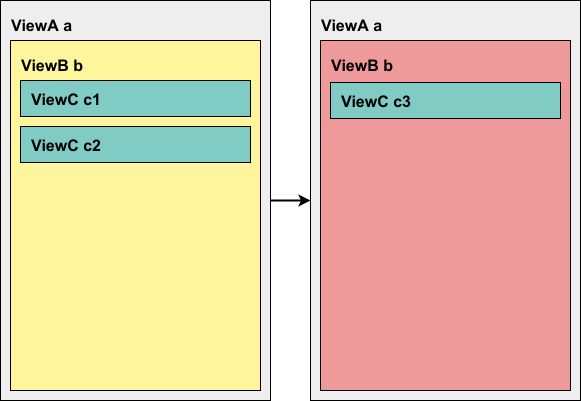
\includegraphics[width=0.8\columnwidth]{declarative_ui_example}
    \caption{Vergleich deklaratives \& imperatives UI}
\end{figure}
\newpage

Im imperativen Stil würde man eine Instanz \textit{b} des so
genannten \textit{Owners} der View \textit{ViewB} nutzen
und mit Hilfe eine Selektors wie beispielsweise \textit{findViewById}
Änderungen auf dieser anwenden (und somit diese implizit invalidieren).
Das kann ungefähr so aussehen:

\begin{figure}[H]
    \centering
    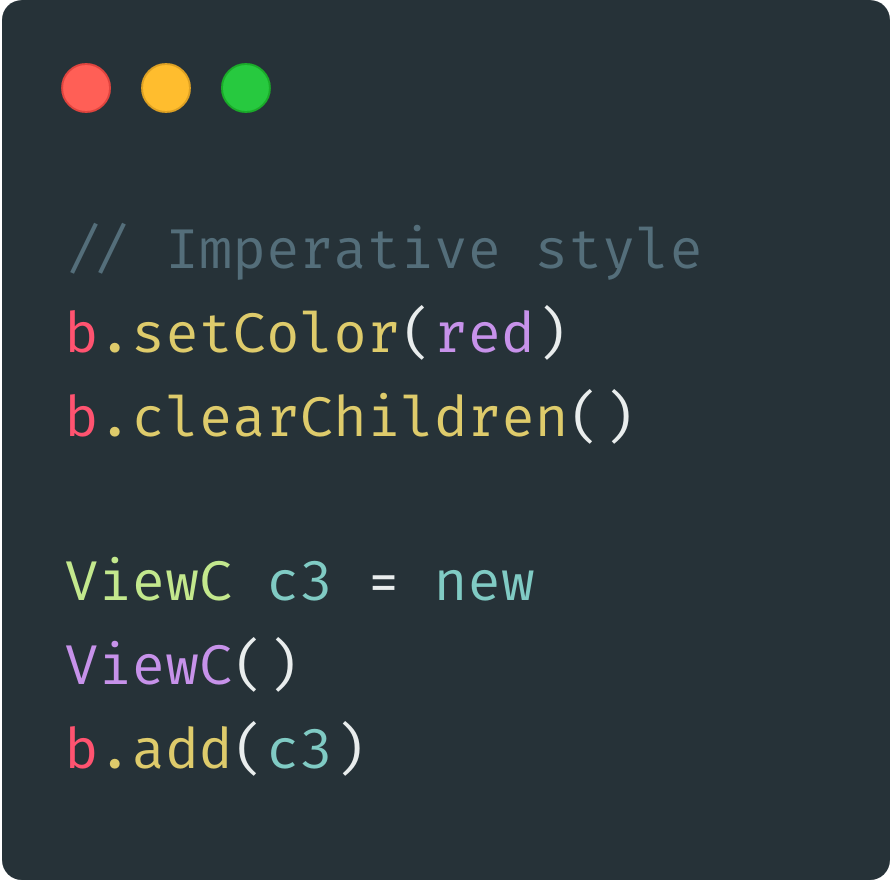
\includegraphics[width=0.4\columnwidth]{imperative_style}
    \caption{Beispiel: imperativer Stil}
\end{figure}

Außerdem müsste dieses Setup im Konstruktor von \textit{ViewB} dupliziert
werden, da die UI (der \ac{SPOT}) möglicherweise die Instanz \textit{b} überlebt.
Im deklarativen Frameworks sind View-Konfigurationen
(wie \textit{Flutter's} Widgets) unveränderlich (immutable) und an sich
nur simple Blaupausen. Um ein UI zu ändern, löst ein Widget einen Rebuild
auf sich selbst aus (in \textit{StatefulWidgets} häufig per \textit{setState()}
und erzeugt damit einen neuen Widget-Subtree.

\begin{figure}[H]
    \centering
    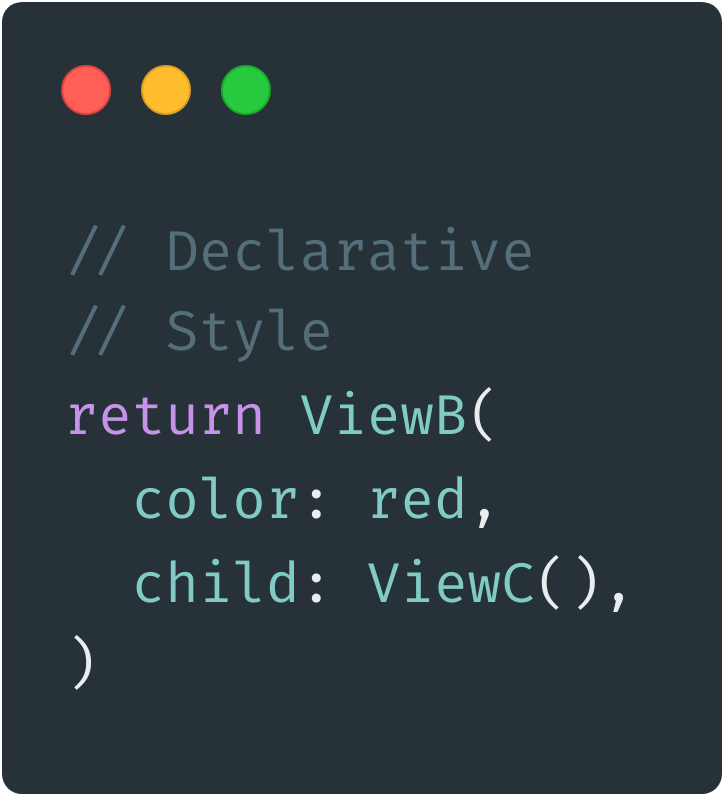
\includegraphics[width=0.4\columnwidth]{declarative_style}
    \caption{Beispiel: deklarativer Stil}
\end{figure}

\section{Herausforderungen}

Die folgenden Abschnitte zeigen Auszüge, die sich bei der Entwicklung
als besonders anspruchsvoll herausgestellt haben.
Dabei werden zum einen technologische als auch Aspekte
des Layouts und Designs betrachtet.

\subsection{Layout \& Design}

Die App besteht grundsätzlich aus drei Bereichen:
einer Liste, einem Informations-Panel und einem Formular.
Diese Bereiche sollen nahtlos ineinander übergehen um ein
möglichst professionellen Gesamteindruck zu vermitteln.
Das finale Layout entspricht in der Hauptansicht der untenstehenden Abbildung.

\begin{figure}[H]
    \minipage[t]{0.4\textwidth}\vspace{0pt}
        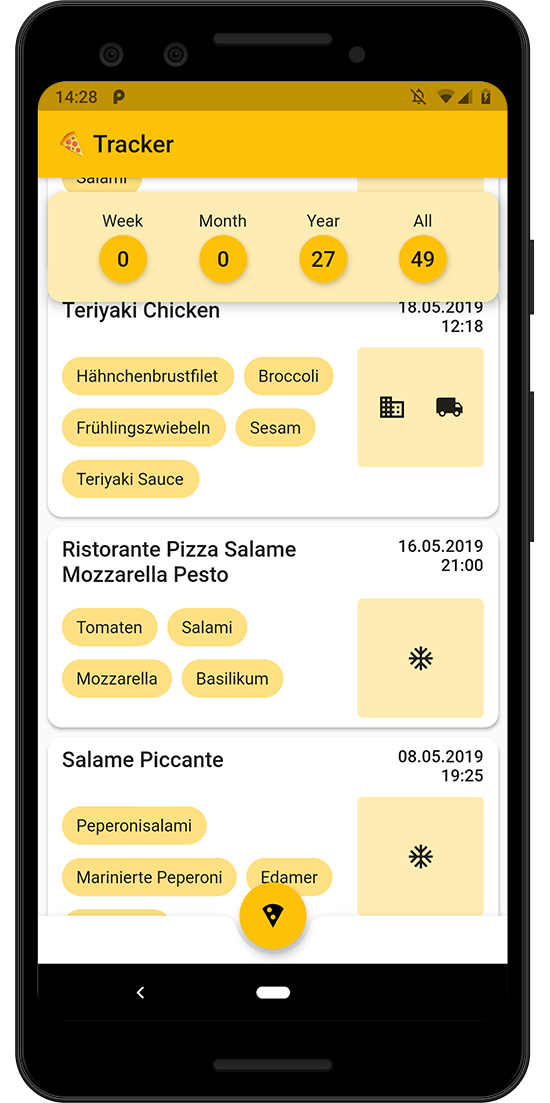
\includegraphics[width=\linewidth]{pixel-3_mockup-1}
        \caption{
            App: Hauptansicht
        }
    \endminipage\hfill
    \minipage[t]{0.6\textwidth}\vspace{0pt}
        Die Anordnung von Elementen erfolgt bei Flutter wie im Web:
        Die Reihenfolge im Quellcode gibt zugleich deren Reihenfolge auf
        der Y-Achse an. Elemente können sich dabei (auf der Z-Achse)
        nicht überlagern. Um Elemente übereinander darzustellen gibt es
        im Web die Property \textit{z-index}, in Flutter nutzt man das Widget
        \textit{Stack}. Im Stack-Widget ist das erste Element das auf der
        Z-Achse niedrigste Element. Grundsätzlich lassen sich viele
        Layout-Konzepte aus dem Web in Flutter übertragen. So gibt es
        Widgets wie \textit{Row, Column, Grid, Flex und Expanded} welche
        in ihrer Funktionalität gleich ihren Web-Pendants entsprechen.
        Interessant ist, dass \textit{Row} allerdings nicht umbricht,
        sobald zu viele Elemente in einer Zeile vorhanden sind und man
        für diesen Fall das Widget \textit{Wrap} benutzen muss.
        Grundsätzlich bietet Flutter eine große Auswahl an Widgets, die über
        reine Layout-Funktionalitäten hinaus gehen und optische Standardwerte
        mit sich bringen. So gibt es das \textit{Card}-Widget welches über
        dessen Properties \textit{elevation} und \textit{shape} einfache
        Mittel bereitstellt, um die Material-Design-typischen Schatten
        und abgerundeten Ecken zu erzielen.

    \endminipage\hfill
\end{figure}
Um nicht nur am oberen, sondern auch am unteren Ende der App
(am sogenannten \ac{FAB}) ein \textit{Überfließen} zu erzielen,
muss die Fläche der Liste auf die komplette Höhe des
Bildschirms erweitert werden.

\begin{figure}[H]
    \minipage[t]{0.4\textwidth}\vspace{0pt}
        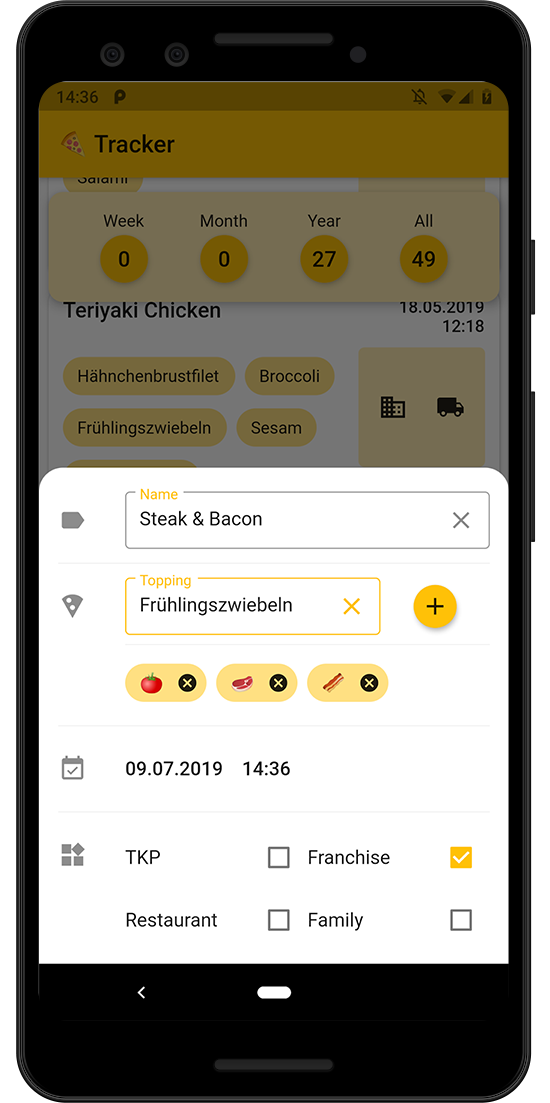
\includegraphics[width=\linewidth]{pixel-3_mockup-2--form}
        \caption{
            App: Formular
        }
    \endminipage\hfill
    \minipage[t]{0.6\textwidth}\vspace{0pt}
        Das Formular an sich besteht mehreren, grundsätzlich
        unabhängigen, Widgets:

        \begin{itemize}
            \itemsep-0.4em
            \item Name
            \item Toppings
            \item Datum \& Uhrzeit
            \item Art der Pizza:
            \begin{itemize}
                \itemsep-0.4em
                \item \ac{TKP}
                \item Franchise
                \item Restaurant
                \item Family
                \item Delivery
                \item Selfmade
            \end{itemize}
            \item Ort an dem die Pizza gegessen wurde
        \end{itemize}

        Hierbei stellten sich vor allem die Widgets für die
        Eingabe der Toppings und der Art der Pizza als besonders
        anspruchsvoll heraus. Bei den Toppings kam zum einen
        zwei Mal das \textit{Row}-, ein Mal das \textit{Wrap}
        sowie für die Toppings selbst das \textit{Chip}-
        (mit \textit{onDeleted}-Methode), bei der
        Art der Pizza vor allem das \textit{Grid}- sowie
        das \textit{Checkbox}- (in Kombination) mit dem \textit{Text}-Widget
        zum Einsatz.
    \endminipage\hfill
\end{figure}
Um im Formular abgerundete Ecken darstellen zu können, benötigt man
das extern erhältliche Widget \textit{showRoundedModalBottomSheet}.
Allerdings kann auch dieses nicht über eine Höhe von 50\% des Bildschirms
hinaus gehen und zwingt einen somit zum scrollen.

\begin{figure}[H]
    \centering
    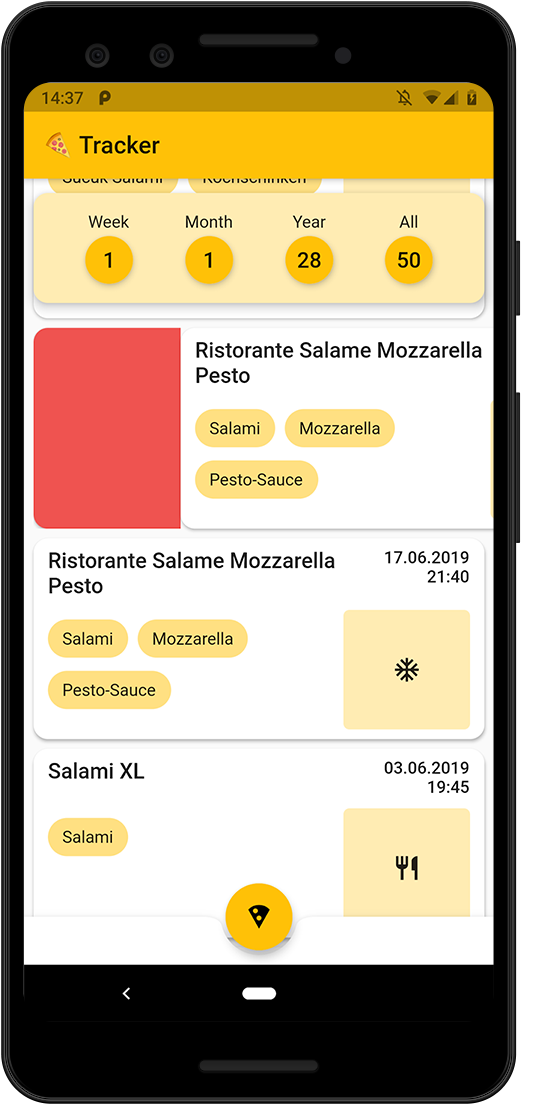
\includegraphics[width=0.4\columnwidth]{pixel-3_mockup-3--dismissible}
    \caption{App: Dismissible}
\end{figure}

Um Pizzen schnell wieder löschen (und später potentiell bearbeiten)
zu können, bietet sich das \textit{Dismissible}-Widget an.
Dieses kann man beliebig um andere Widgets packen und diesem
durch wischen in bestimmte Richtungen verschiedene Aktionen zuweisen.
\newpage

\subsection{Daten zwischen Widgets teilen}
Aufgrund der Art und Weise wie \textit{Flutter} entworfen wurde,
können Daten zwischen Widgets nur von oben nach unten
beziehungsweise vom Eltern- zum Kind-Widget übergeben werden.
In der unten stehenden Abbildung ist das Eingabeformular der App zu sehen.
Dieses besteht wie bereits erwähnt aus verschiedenen Widgets.
Jede \textit{"Zeile"} ist ein Widget und enthält wiederum Widgets
wie Formularfelder, \textit{Checkboxen} oder \textit{Chips}.
Auf der Ebene des Formulars selbst, aber in der Abbildung nicht zu sehen,
ist der Button zum senden der Daten. Würde das Formular ausschließlich
aus Formularfeldern bestehen, wäre dies auch kein größeres Problem.
In diesem Fall könnte man auf sämtliche Formularfelder direkt zugreifen.
Jedoch besteht das Formular auch aus solchen Widgets die Listen
repräsentieren und keine klassischen Formularfelder sind.
Diese beiden Bereiche sind in der Abbildung cyanfarben umrandet.
Zum einen kann eine Pizza mehrere Toppings und zum anderen
gleichzeitig verschiedene Typen annehmen.

\begin{figure}[H]
    \centering
    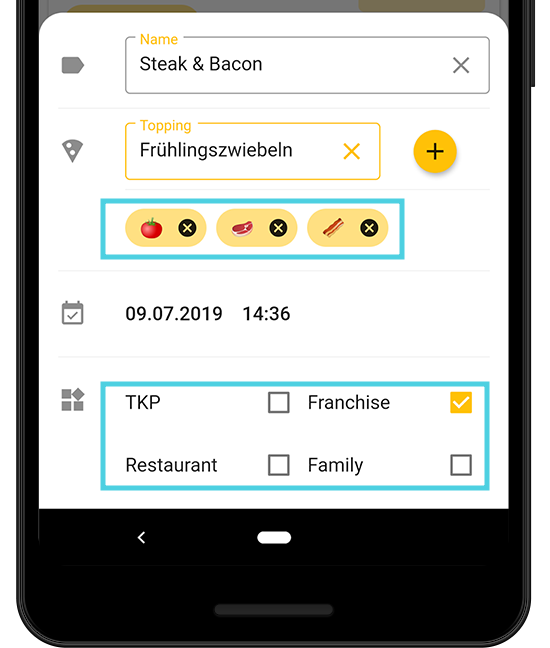
\includegraphics[width=0.4\columnwidth]{pixel-3_mockup-4--shared-data}
    \caption{App: Formular mit Shared-Data}
\end{figure}

Da diese Listen eine Ebene tiefer als der Button zum Absenden der Daten liegen,
kann es keinen direkten Zugriff geben.
In \textit{Flutter} gibt es grundsätzlich zwei Arten wie Daten übergeben werden können:

\begin{enumerate}
    \itemsep-0.4em
    \item Daten über den Konstruktor des Widgets hinzufügen
    \item \textit{Flutter}'s \textit{BuildContext}
\end{enumerate}

\newpage

Jedem Widget steht die Klasse \textit{BuildContext} zur Verfügung.
Diese erlaubt es einem Widget, mit Hilfe der folgenden Methoden
Daten von jedem Vorfahren anzufordern.

\begin{itemize}
    \itemsep-0.4em
    \item \textit{inheritFromWidgetOfExactType(Type)}
    \item \textit{ancestorStateOfType(TypeMatcher)}
    \item \textit{ancestorWidgetOfExactType(Type)}
\end{itemize}

Besonders abfrageintensiven Operationen empfiehlt
sich \textit{inheritFromWidgetOfExactType(Type)}.
Diese Methoden gehören zur Basis-Klasse \textit{InheritedWidget}.
Solche \textit{Inherited}-Widgets lösen einen Rebuild im Konsumenten
aus wenn deren State geändert wurde.
Um das Handling mit diesen Methoden zu vereinfachen,
nutze ich das Paket \textit{provider}. Welches vor allem
\textit{Syntax Sugar} für \textit{InheritedWidget} bietet.
Um Daten einfach zwischen Widgets teilen zu können,
empfiehlt es sich, sogenannte Daten-Klassen zur
Haltung sowie Manipulation dieser zu vereinfachen.
Dies kann nach folgendem Muster gelöst werden:

\begin{figure}[H]
    \centering
    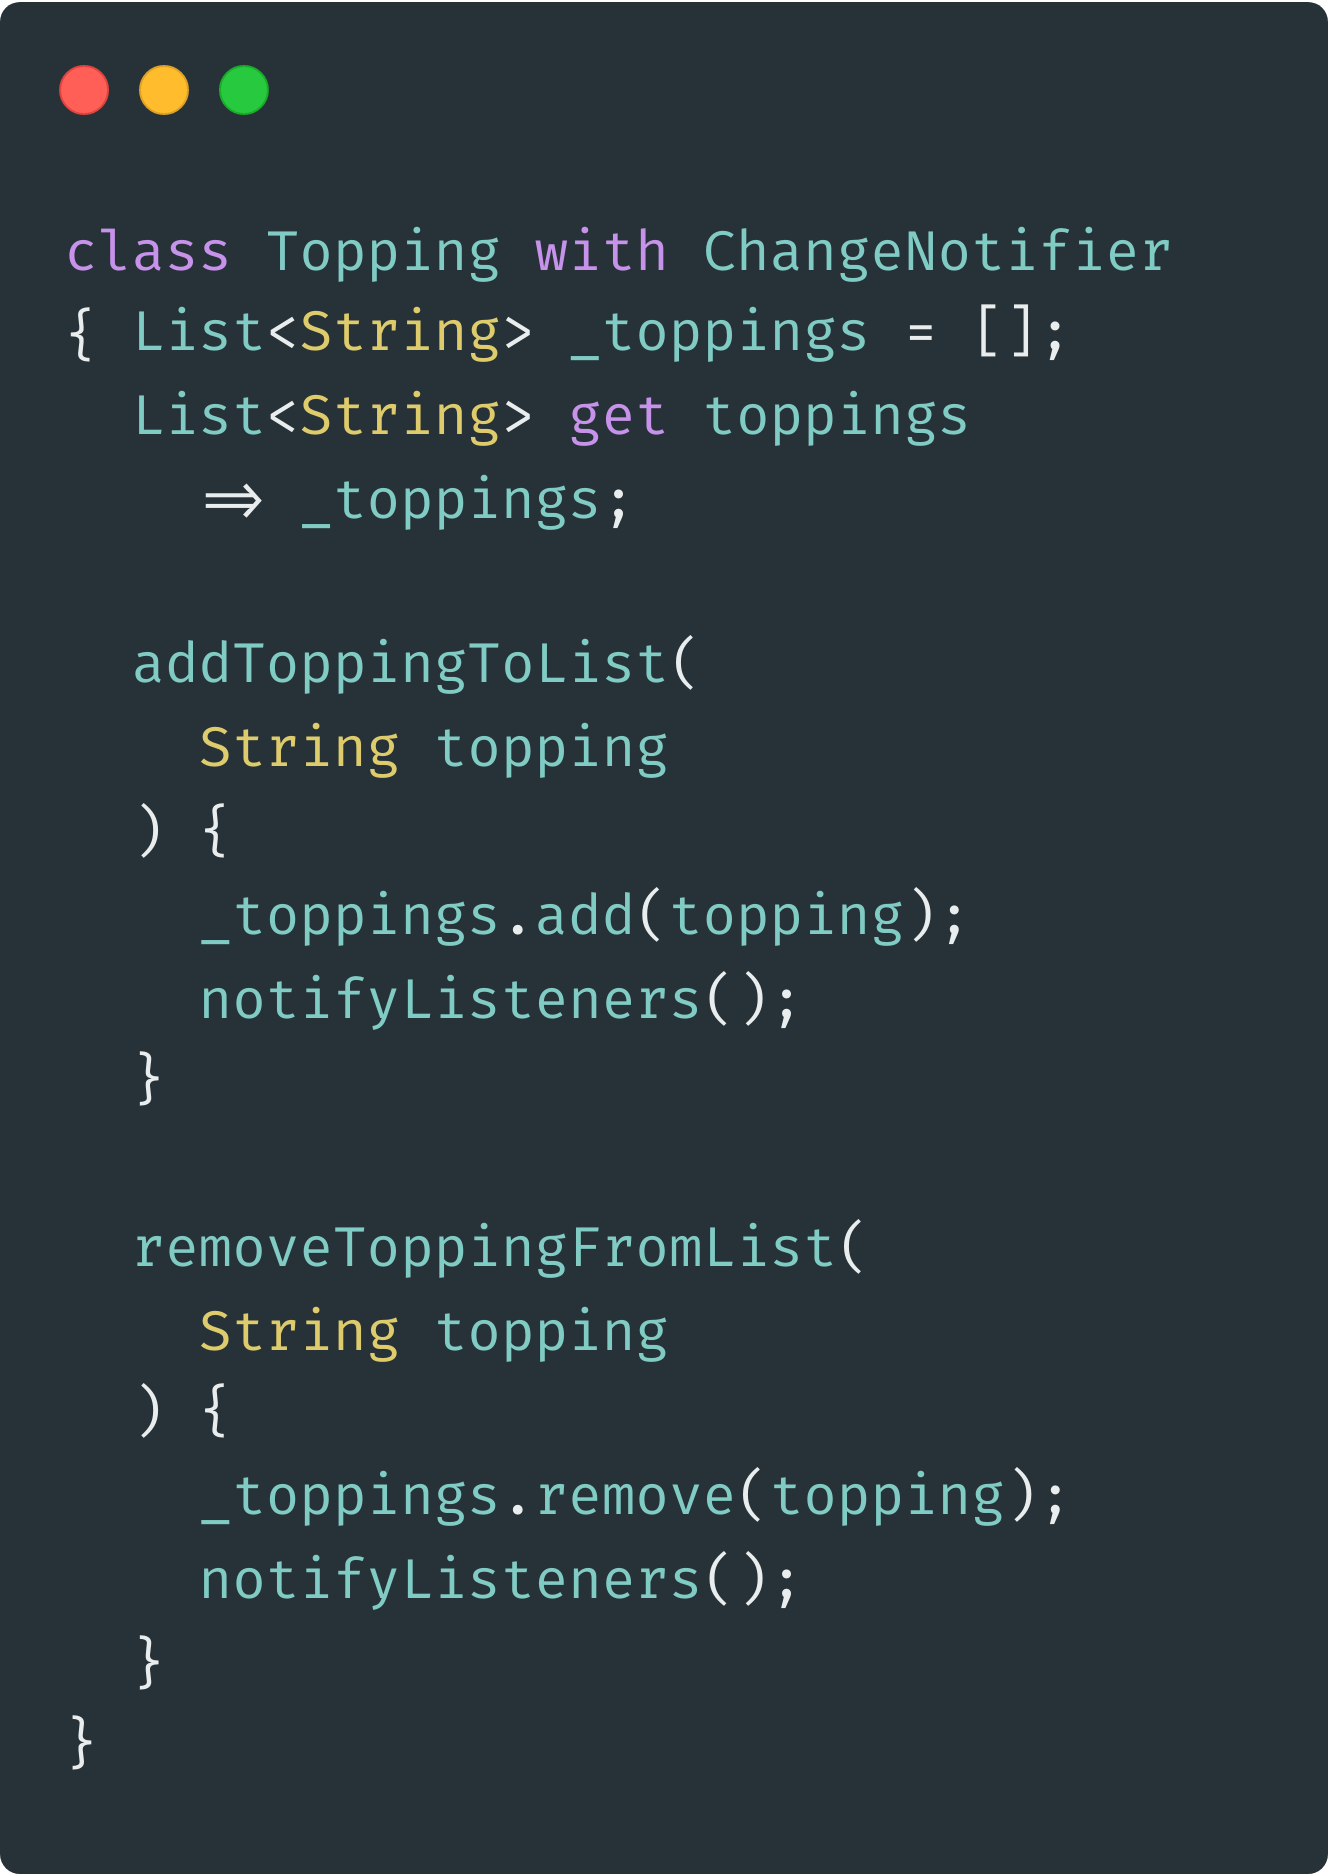
\includegraphics[width=0.4\columnwidth]{topping_change-notifier}
    \caption{Dart: ChangeNotifier}
\end{figure}

Über das sogenannte \textit{Mixin "ChangeNotifier"} lassen
sich Eigenschaften und Methoden dieser Klasse auf die eigene Daten-Klasse
übertragen. Die in den Methoden \textit{addToppingToList} \& \textit{removeToppingToList}
aufgerufene Methode \textit{notifyListeners} informiert das Formular immer dann darüber,
dass Änderungen an den Listen stattgefunden haben.
Somit ändert sich der State der Widgets an sich sowie des Formulars, welches wiederum
einen Rebuild auslöst.
Um diese Daten-Klassen dann im Formular nutzen zu können,
müssen die Provider eine Ebene höher, in diesem Fall in der \textit{main.dart}
wie folgt eingebunden werden:

\begin{figure}[H]
    \centering
    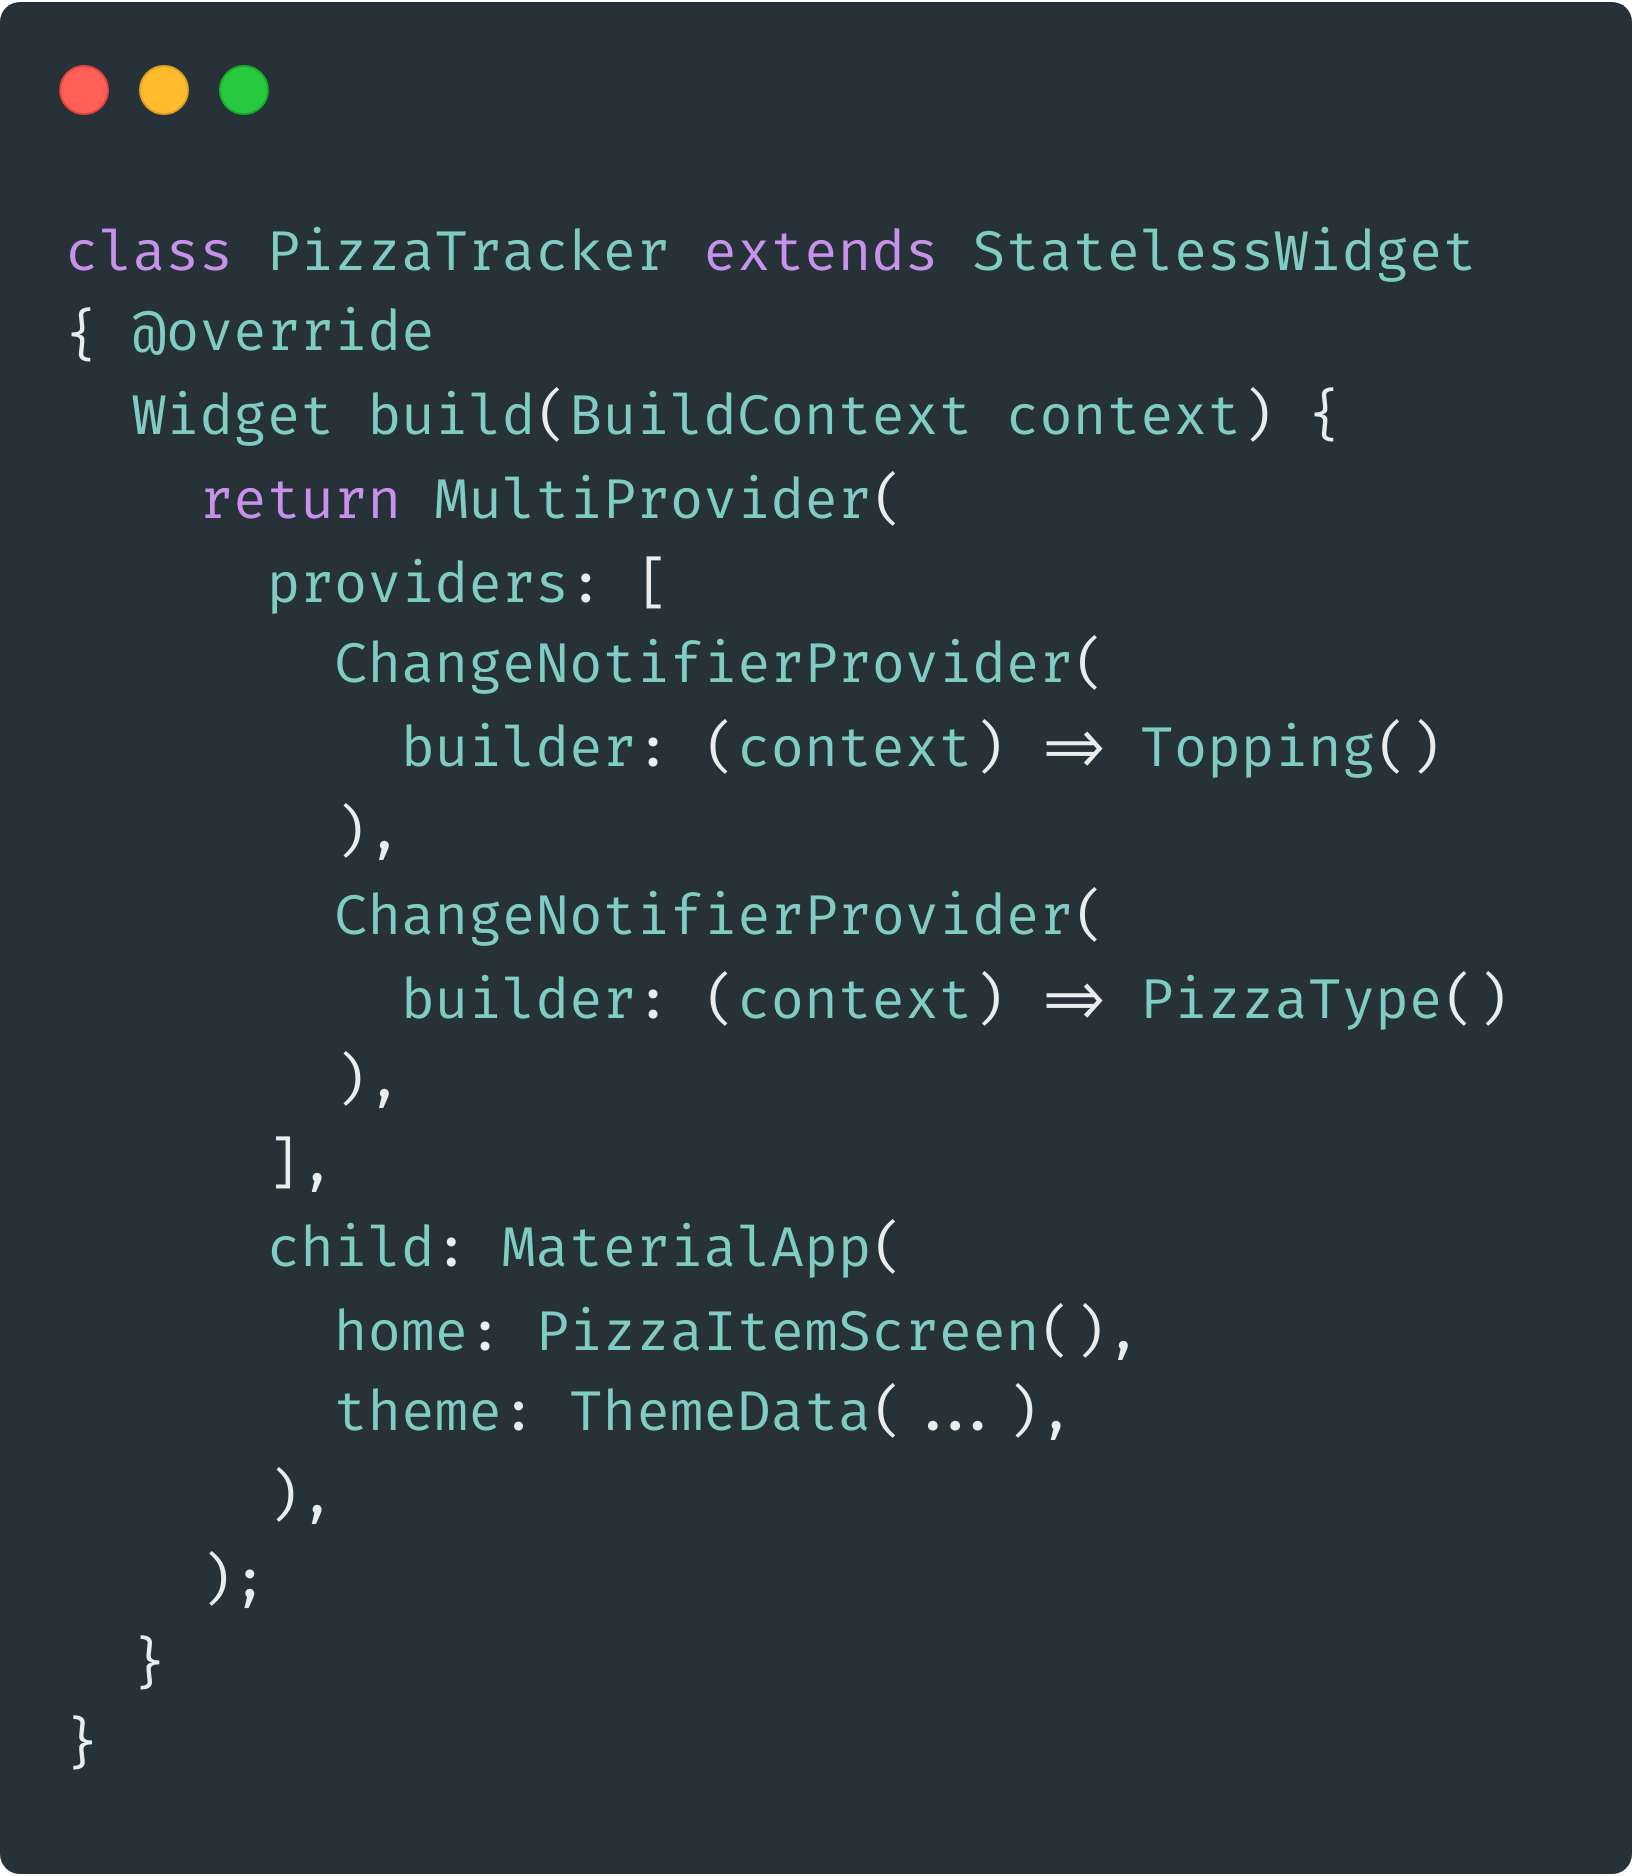
\includegraphics[width=0.4\columnwidth]{multi_provider}
    \caption{Dart: MultiProvider}
\end{figure}

\newpage

\subsection{Fehlende Date-Library}

Um Filter für die verschiedenen Zeiträume setzen zu können,
ist es notwendig, ausgehend vom jetzigen Zeitpunkt,
den jeweiligen Start- und Endpunkt eines Zeitraums zu ermitteln.
Wichtig bei der Berechnung von Zeiträumen ist unter anderem auch
die korrekte Einbeziehung der Umstellung von Sommer- und Winterzeit
oder ob eine Woche an einem Sonntag oder Montag beginnt.
Im Web gibt es für solche und ähnliche Berechnungen Bibliotheken
wie beispielsweise \href{https://momentjs.com/docs/}{\textit{Moment.js}}
oder \href{https://date-fns.org/}{\textit{date-fns}}.
Solch eine Bibliothek gibt es allerdings noch nicht im Dart-/Flutterkosmos.
Dementsprechend schrieb ich verschiedene Utility-Funktionen wie
beispielsweise folgende um den letzten Tag eines Monats zu erhalten:
\begin{figure}[H]
    \centering
    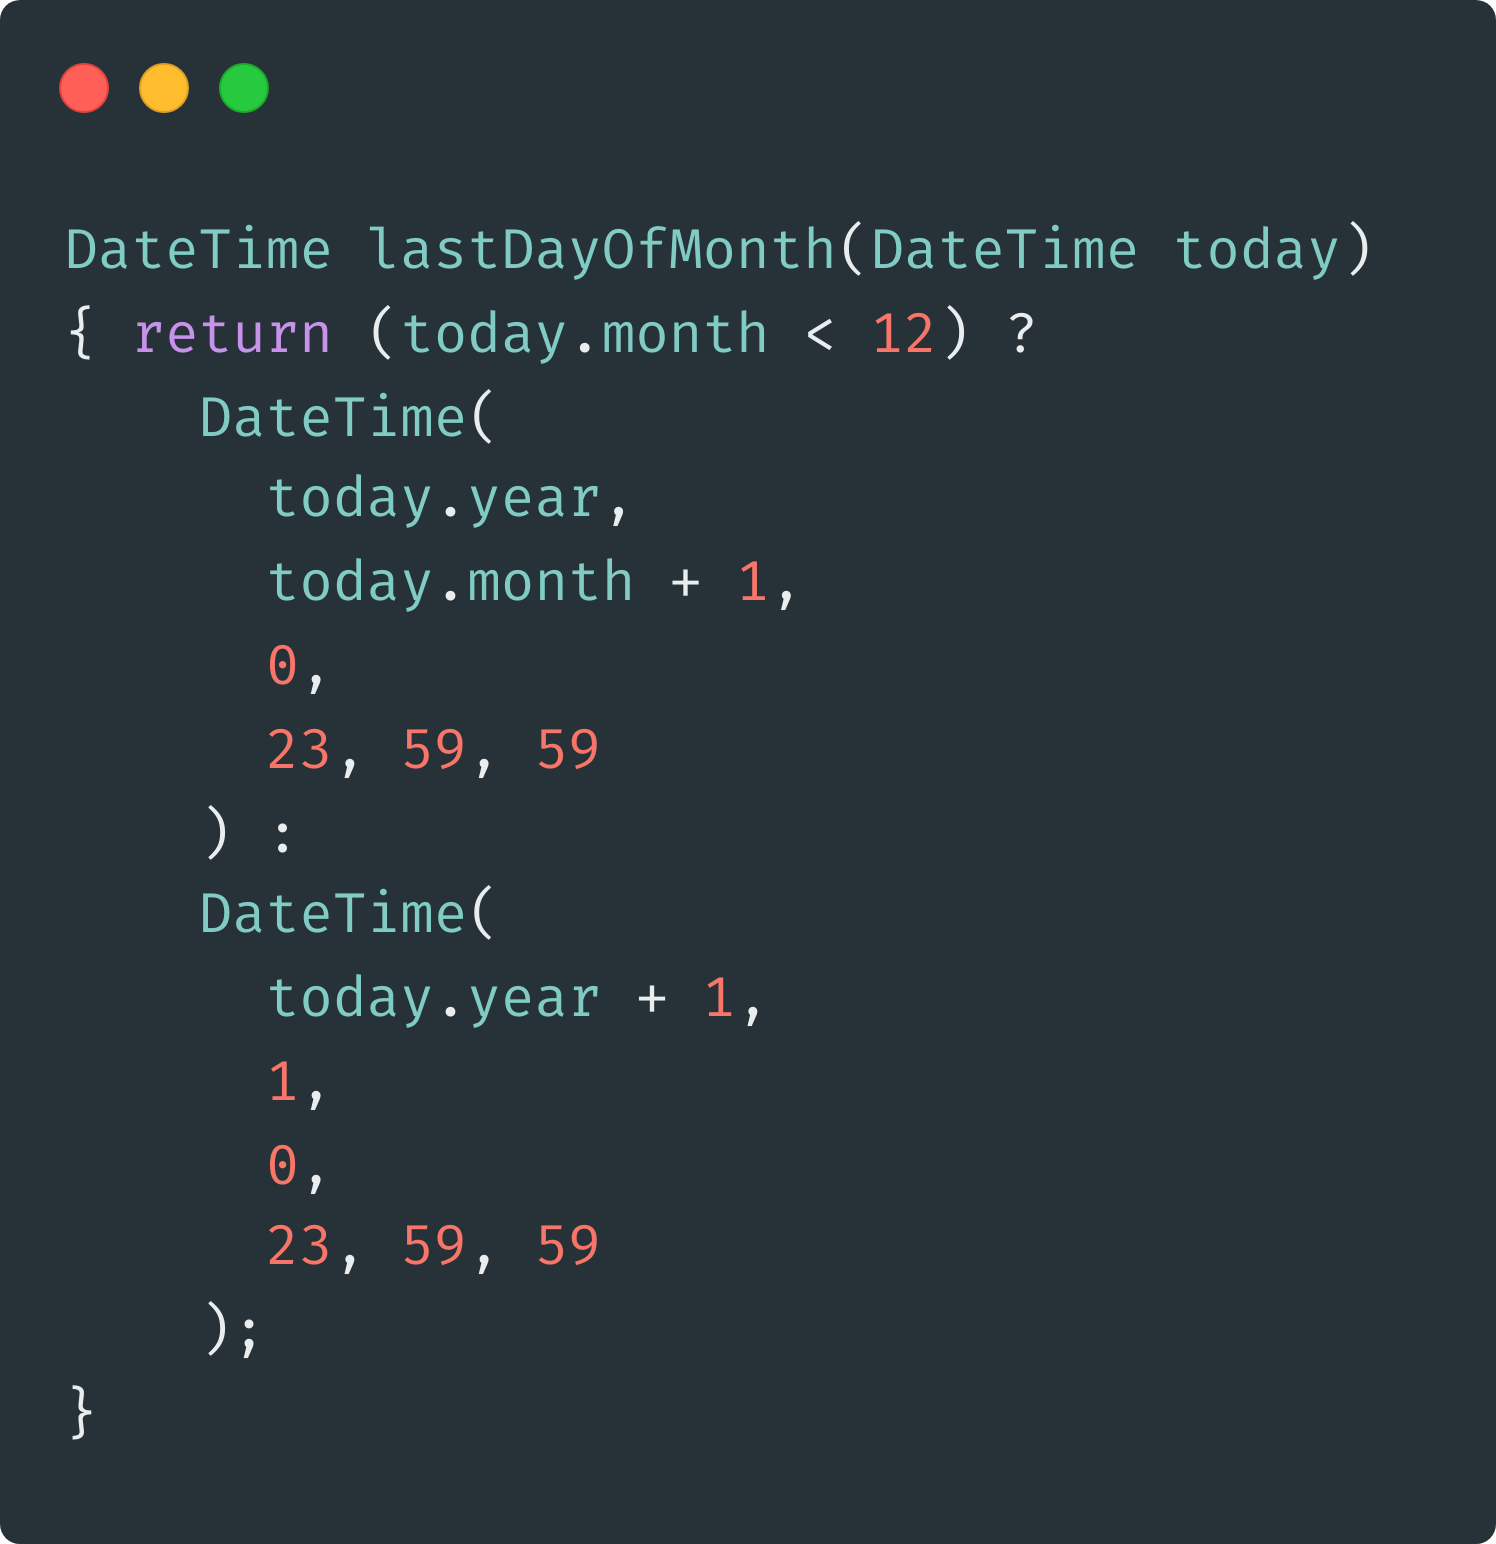
\includegraphics[width=0.4\columnwidth]{last_day_of_month}
    \caption{Dart: Letzter Tag des Monats}
\end{figure}


\section{Fazit}

Die Entwicklung einer App mit \textit{Flutter}
brachte eine steile Lernkurve mit sich und bot
eine neue Sicht auf bereits bekannte Konzepte.
Als besonders herausfordernd stellte sich die
Einarbeitung und Umsetzung von Layout und Design
heraus. Auch das verhältnismäßig junge Alter
des Frameworks brachte Herausforderungen mit sich;
nicht immer gibt es aus anderen Frameworks bekannte
Bibliotheken oder entsprechende Tutorials oder
Blogbeiträge um sich Wissen neben der üblichen
Dokumentation anzueignen. In diesem Projekt nicht
betrachtet wurde die Cross-Plattform-Funktionalität
mit der auch \textit{iOS}-Apps entwickelt werden können.
Alles in allem war dieses Projekt,
auch wenn mit einem zwinkernden Auge zu sehen,
sehr lehrreich und spaßig umzusetzen.

\newpage

% Don't use page-numbers from here on
% \pagenumbering{gobble}
% \raggedright
\begin{thebibliography}{xxxxxxxxxxxxxxxxxxxxxxxxxxxxxxxxxxxx}
    \bibitem
        [Steve Krug, 2014]
        {bmbf} Don't Make Me Think! Revisited - Das intuitive Web
    \bibitem
        [Jens Jacobsen, Lorena Meyer, 2017]
        {bmbf} Praxisbuch Usability und UX: Was jeder wissen sollte,
        der Websites und Apps entwickelt - bewährte Methoden praxisnah erklärt
    \bibitem
        [Google, 2018]
        {bmbf} Angular,
        verfügbar unter: \url{https://angular.io/}\\

        Material Design,
        verfügbar unter: \url{https://material.io/design/}\\

        Material Design Components Web,
        verfügbar unter: \url{https://material.io/develop/web/}
    \bibitem
        [Dominic Carretto, 2018]
        {bmbf} Material Design Components for Angular,
        verfügbar unter:\\ \url{https://trimox.github.io/angular-mdc-web/#/home}
    \bibitem
        [Tony Spegel, 2018]
        {bmbf} Free-Rooms-Py,
        verfügbar unter:\\ \url{https://github.com/TonySpegel/free-rooms-py}\\

        Free-Rooms 2.0 "Snegon",
        verfügbar unter: \url{https://github.com/TonySpegel/Snegon}
\end{thebibliography}


\end{document}
